\documentclass{ximera}
\title{Image and Alt text}

\input{imagePreamble}% Only add a preamble file if it is actually necessary for the demo/test.
\begin{document}
\begin{abstract}
    Testing/demo for alt text in documents.
\end{abstract}
\maketitle

% In case using this with an old ximeraLatex ...
\providecommand{\xmalt}[1]{WARNING: Using LOCAL xmalt command with arg #1}

A TikZ image in an image environment:
\begin{image}[0.3\textwidth]
    \alt{A sine function forms a wave shape (alt text with alt comman, inside image environment)}
    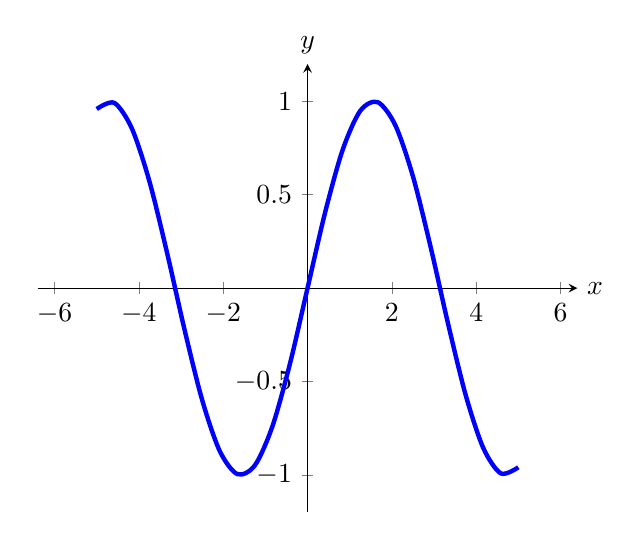
\begin{tikzpicture}
      \begin{axis}[
          xmin=-6.4,
          xmax=6.4,
          ymin=-1.2,
          ymax=1.2,
          axis lines=center,
          xlabel=$x$,
          ylabel=$y$,
          every axis y label/.style={at=(current axis.above
              origin),anchor=south},
          every axis x label/.style={at=(current axis.right of
              origin),anchor=west},
        ]
        \addplot [ultra thick, blue, smooth] {sin(deg(x))};
      \end{axis}
    \end{tikzpicture}
  \end{image}

  \xmalt{A sine function forms a wave (alt text with with command xmalt)}

A PNG in an image environment:
\begin{image}[0.3\textwidth]
    \alt{The ximera logo (this is the alt text from the alt command, inside an image environment)}
    
\includegraphics[alt={The Ximera Logo (this is the alt text of includegraphics)}]{missionPatch.png}
\end{image}
\undef\xmaltprint   %% This should make the \xmalt text NOT TO BE PRINTED IN THE PDF
\xmalt{The ximera logo (this is the alt text from the xmalt command)}


\end{document}
